\documentclass[a4paper,12pt]{article}

\usepackage[margin=2cm]{geometry}

\usepackage{graphicx}

% For cross-referencing
\usepackage{xr}
\externaldocument{main_plos}
\externaldocument[S1.]{S1_Text}
\externaldocument[S2.]{S2_Text}
\externaldocument[S3.]{S3_Text}
\externaldocument[S4.]{S4_Text}


% Caption package for small captions option
% ... convenient to list figures during manuscript processing
\usepackage{caption}
% Language and fonts
\usepackage[english]{babel}
\usepackage[T1]{fontenc}
\usepackage[utf8]{inputenc}

% Math Stuff
\usepackage{amsmath,amsfonts}
\newcommand{\argmax}{\operatornamewithlimits{argmax}}
\newtheorem{theorem}{Theorem}

% Chemical Stuff
\usepackage[version=3]{mhchem}

\usepackage{hyperref}
% Add an S1
\renewcommand{\thetable}{S1.\arabic{table}}%
\renewcommand{\thefigure}{S1.\arabic{figure}}%
\renewcommand{\theequation}{S1.\arabic{equation}}
\renewcommand{\thesection}{S1.\arabic{section}}%

\usepackage{color} 
\newcommand{\tr}[1]{{#1}}

\begin{document}

\begin{flushleft}
{\Large
\textbf\newline{\textbf{S1 Text -- Model derivation and analysis\footnote{Supporting Information of "Dynamical Allocation of Cellular Resources as an Optimal Control Problem: Novel Insights into Microbial Growth Strategies"}}}
}
\newline
% Insert author names, affiliations and corresponding author email (do not include titles, positions, or degrees).
\\
Nils Giordano \textsuperscript{1,3},
Francis Mairet \textsuperscript{2},
Jean-Luc Gouzé \textsuperscript{2},
Johannes Geiselmann \textsuperscript{1,3,*},
Hidde de Jong \textsuperscript{3,*}
\\
\bigskip
\bf{1} Université Grenoble Alpes, Laboratoire Interdisciplinaire de Physique (CNRS UMR 5588), 140 rue de la Physique BP 87, 38402 Saint Martin d'Hères, France
\\
\bf{2} Inria, Sophia-Antipolis Méditerranée research centre, 2004 route des Lucioles, BP 93, 06902 Sophia-Antipolis Cedex, France
\\
\bf{3} Inria, Grenoble - Rhône-Alpes research centre, 655 avenue de l'Europe, Montbonnot, 38334 Saint Ismier Cedex, France
\\
\bigskip

* Corresponding authors with equal contributions:\\
Hidde.de-Jong@inria.fr, Hans.Geiselmann@ujf-grenoble.fr
\end{flushleft}

\section{Model formulation}

The time evolution of the total mass of each component of the self-replicator can be written as follows:
\begin{eqnarray}
\frac{dP}{dt} &=& V_M(t) - V_R(t) \nonumber , \\
\frac{dM}{dt} &=& (1-\alpha(t))\, V_R(t) \label{eq:ext_system},\\
\frac{dR}{dt} &=& \alpha(t) \, V_R(t)  \nonumber ,
\end{eqnarray}
where $P$, $M$, $R$ [g] denote the total mass of precursors, metabolic machinery and gene expression machinery, respectively.
$V_M$ [g h$^{-1}$] is the rate of production of precursors by metabolism and $V_R$ [g h$^{-1}$] the rate of utilisation of precursors for gene expression.

Dividing the mass variables by the total time-varying volume $\texttt{Vol}(t)$ of the system, we obtain the concentration variables $p = P/\texttt{Vol}$, $m = M/\texttt{Vol}$, $r = R/\texttt{Vol}$ [g L$^{-1}$].
The dynamics of the concentration variables then follows with Eq.~\ref{eq:ext_system}:
\begin{eqnarray}
\frac{dp}{dt} &=& \frac{V_M(t)}{\texttt{Vol}} - \frac{V_R(t)}{\texttt{Vol}} - \frac{1}{\texttt{Vol}}\frac{d\texttt{Vol}}{dt}\, p, \nonumber \\
\frac{dm}{dt} &=& (1-\alpha(t)) \frac{V_R(t)}{\texttt{Vol}} - \frac{1}{\texttt{Vol}}\frac{d\texttt{Vol}}{dt} \, m  \label{eq:deriv_int_system},\\ 
\frac{dr}{dt} &=& \alpha(t) \, \frac{V_R(t)}{\texttt{Vol}}  - \frac{1}{\texttt{Vol}}\frac{d\texttt{Vol}}{dt} \, r. \nonumber
\end{eqnarray}

At this point, we define $v_M = V_M/\texttt{Vol}$ and $v_R = V_R/\texttt{Vol}$ [g L$^{-1}$ h$^{-1}$] as the mass fluxes per unit volume.
Moreover, with the definition of the volume in terms of the total protein mass in Eq.~\ref{eq:voldef} of the main text, that is, $\texttt{Vol} = \beta\, (M + R)$, we find that
\begin{equation}
\label{eq:supp_deriv_growthrate}
\frac{1}{\texttt{Vol}} \frac{d\texttt{Vol}}{dt} = \frac{\beta}{\texttt{Vol}} \frac{d(M+R)}{dt} = \beta\, \frac{V_R(t)}{\texttt{Vol}} = \beta \, v_R(t).
\end{equation}
This leads to the system
\begin{eqnarray}
\frac{dp}{dt} &=& v_M(t) - v_R(t) \, (1+\beta\, p), \label{eq:supp_pdef}\\
\frac{dr}{dt} &=& v_R(t)  \, (\alpha(t) - \beta\, r) \label{eq:supp_rdef},
\end{eqnarray}
where the equation for $m(t)$ is omitted since by construction $r(t) + m(t) = 1/\beta$ and $dr/dt + dm/dt = 0$.

As stated in the main text, we use Michaelis-Menten kinetics to express $v_M$ and $v_R$ in terms of the system variables:
\begin{eqnarray}
v_M(t) &=& m(t) \, k_M \, \frac{s(t)}{K_M +s(t)} = \left(\frac{1}{\beta} - r(t)\right)\, e_M(t) \nonumber, \\
v_R(t) &=& r(t) \, k_R \, \frac{p(t)}{K_R +p(t)}, \nonumber 
\end{eqnarray}
with rate constants $k_M$, $k_R$ [h$^{-1}$] and half-saturation constants $K_M$, $K_R$ [g L$^{-1}$].
$s(t)$ is an exogenous variable representing the nutrient concentration in the external medium.
We simplify $v_M(t)$ by defining the environmental input $e_M(t) = k_M \, s(t) / (K_M + s(t))$.
\tr{Throughout the paper, as explained in the main text, we assume the environment is constant, \textit{i.e.}, $e_M(t)=e_M$.}

Finally, the growth rate $\mu$ [h$^{-1}$] is defined as the relative increase of the volume of the self-replicator.
From Eq.~\ref{eq:supp_deriv_growthrate}, it follows that:
\begin{equation}
\label{eq:supp_growthrate}
\mu (t) = \frac{1}{\texttt{Vol}} \frac{d\texttt{Vol}}{dt} = \beta\, v_R(t).
\end{equation}

\section{Nondimensionalization of the system}

For the sake of simplifying the proofs and derivations below, we define the following nondimensional variables:
\begin{equation*}
\hat{p}  = \beta \, p,\;\;\;
\hat{r}  = \beta \, r,\;\;\;
\hat{t}  = k_R \, t.
\end{equation*}
When injecting these into Eq.~\ref{eq:supp_pdef}, we obtain
\[
\frac{k_R}{\beta} \, \frac{d\hat{p}}{d\hat{t}} = \left( \frac{1}{\beta} - \frac{\hat{r}}{\beta} \right) \, e_M - \frac{\hat{r}}{\beta} \, k_R \, \frac{\hat{p}}{\beta K_R + \hat{p}} \, (1 + \hat{p}),
\]
which simplifies to
\[
\frac{d\hat{p}}{d\hat{t}} = ( 1 - \hat{r} ) \, \frac{e_M}{k_R} - \hat{r} \, \frac{\hat{p}}{\beta K_R + \hat{p}} \, (1 + \hat{p}).
\]
In a similar manner, we derive the time evolution of the nondimensional $\hat{r}$, and thus obtain the system
\begin{equation}
\label{eq:supp_adim}
\begin{aligned}
\frac{d\hat{p}}{d\hat{t}} &= (1-\hat{r})\, E_M - (1 + \hat{p}) \, \frac{\hat{p}}{K + \hat{p}}\, \hat{r},\\
\frac{d\hat{r}}{d\hat{t}} &= (\alpha - \hat{r}) \, \frac{\hat{p}}{K + \hat{p}}\, \hat{r},
\end{aligned}
\end{equation}
with the lumped parameters $E_M = e_M / k_R$ and $K = \beta \, K_R$.
The corresponding nondimensionalized growth rate is given by
\begin{equation}
\label{eq:supp_growthrate_adim}
\hat{\mu} = \frac{\mu}{k_R} = \frac{\hat{p}}{K+\hat{p}} \, \hat{r}.
\end{equation}

\section{Steady-state growth of the self-replicator}
\label{si::growthrate}

If we suppose $E_M > 0$, $K > 0$ and $\alpha \in ]0, 1[$, there is a trivial unstable steady state at $(0, 1)$.
A second steady-state exists for the point in which $\hat{r}^* = \alpha$ and $\hat{p}^*$ is a root of the following polynomial:
\[
\alpha \, \hat{p}^2 + \left(\alpha - (1-\alpha) \, E_M \right) \hat{p} - (1-\alpha)\, E_M\, K.
\]
If we keep the only admissible root for this polynomial (\textit{i.e.}, for which $\hat{p} \geq 0$), the second steady state is given by
\begin{equation}
\label{eq:supp_steadystate}
(\hat{p}^*, \hat{r}^*) = \left( \frac{(1-\alpha)\, E_M - \alpha + \sqrt{[(1-\alpha)\, E_M - \alpha]^2 + 4\alpha\, (1-\alpha)\, E_M\, K}}{2\alpha}, \alpha \right).
\end{equation}
We can determine the stability of this steady state by looking at the Jacobian matrix $J$ of the ODE system:
\begin{equation}
\label{eq:supp_jacop}
J = \left(\begin{matrix}
- \frac{\hat{r}}{K + \hat{p}} \left[ \hat{p} + (1+\hat{p})\, \frac{K}{K+\hat{p}}\right] & - E_M - (1+\hat{p})\frac{\hat{p}}{K+\hat{p}}\\
(\alpha - \hat{r})\, \hat{r} \, \frac{K}{(K+\hat{p})^2} & (\alpha - 2\hat{r})\, \frac{\hat{p}}{K+\hat{p}}
\end{matrix}\right) .
\end{equation}
Evaluated at the point $(\hat{p}^*, \hat{r}^*)$, the Jacobian matrix becomes
\[
J_{(\hat{p}^*, \hat{r}^*)} = \left(\begin{matrix}
- \frac{\alpha}{K + \hat{p}^*} \left[ \hat{p}^* + (1+\hat{p}^*)\frac{K}{K+\hat{p}^*}\right] & - E_M - (1+\hat{p}^*)\frac{\hat{p}^*}{K+\hat{p}^*}\\
0 & -\alpha\frac{\hat{p}^*}{K+\hat{p}^*}
\end{matrix}\right).
\]
Since $\hat{p}^*$, $\alpha$, $E_M$, $K$ $>0$, the two eigenvalues are negative and therefore the steady state $(\hat{p}^*, \hat{r}^*)$ is stable (see also the streamlines in Figure~\ref{fig:model_analysis}\textit{A} in the main text).
It means that for fixed environmental conditions $E_M$ and resource allocation $\alpha$, the self-replicator converges towards a steady state in which the concentration variables are constant.

One can now easily derive the steady-state growth rate, denoted $\hat{\mu}^*$.
By substituting Eq.~\ref{eq:supp_growthrate_adim} into the first ODE of the system of Eq.~\ref{eq:supp_adim}, we find at steady state:
\[
\left(\frac{d\hat{p}}{d\hat{t}}\right)_{(\hat{p}^*, \hat{r}^*)} = 0 = (1-\alpha)\, E_M - (1+\hat{p}^*)\, \hat{\mu}^*,
\]
which by means of Eq.~\ref{eq:supp_steadystate} gives the following relation:
\begin{equation}
\label{eq:supp_growthrate_p}
\hat{\mu}^* = \frac{(1-\alpha)\, E_M}{1+\hat{p}^*} = \frac{2\alpha(1-\alpha)\, E_M}{(1-\alpha)\, E_M + \alpha + \sqrt{\left[(1-\alpha)\, E_M -\alpha\right]^2 + 4\alpha(1-\alpha)\, E_M\, K}}.
\end{equation}
Finally, we can transform this expression to obtain
\begin{equation}
\label{eq:supp_growthrate_final}
\hat{\mu}^* = \begin{cases}
\frac{(1-\alpha)\, E_M + \alpha - \sqrt{\left[(1-\alpha)\, E_M - \alpha\right]^2 + 4(1-\alpha)\, \alpha\, E_M\, K}}{2(1-K)} &\text{ for }K\neq 1,\\
\frac{\alpha\, (1-\alpha)\, E_M}{\alpha + (1-\alpha)\, E_M} &\text{ for }K = 1.
\end{cases}
\end{equation}
This function of $\alpha$ is plotted in Figure~\ref{fig:model_analysis}\textit{B} in the main text.

\section{Maximization of growth rate at steady state}
\label{si::optimal}

We are interested in the steady state at which growth occurs at the maximum rate.
The growth rate at steady state $\hat{\mu}^*$ is given by
\begin{equation}
\label{eq:supp_growthrate_steadystate}
\hat{\mu}^* = \frac{\hat{p}^*}{K + \hat{p}^*} \, \hat{r}^* .
\end{equation}
From the first ODE of the system of Eq.~\ref{eq:supp_adim}, we have
\begin{equation}
\label{eq:supp_isop}
\hat{r}^* = \frac{E_M}{E_M + \frac{\hat{p}^*}{K + \hat{p}^*} (1+\hat{p}^*)} .
\end{equation}
Substituting Eq.~\ref{eq:supp_isop} into Eq.~\ref{eq:supp_growthrate_steadystate}, we obtain
\begin{equation}
\label{eq:supp_growthrate_steadystate_p}
\hat{\mu}^* = \frac{E_M \, \hat{p}^*}{\hat{p}^{* 2} + (E_M + 1)\, \hat{p}^* + E_M\, K} .
\end{equation}
The value of $\hat{p}^*$ maximizing $\hat{\mu}^*$ can be determined from
\begin{equation}
\label{eq:supp_growthrate_steadystate_deriv_p}
\frac{\partial\hat{\mu}^*}{\partial\hat{p}^*} = \frac{E_M \, (E_M\, K - \hat{p}^{*2})}{\left(\hat{p}^{* 2} + (E_M + 1)\, \hat{p}^* + E_M\, K\right)^2},
\end{equation}
by looking at the values of $\hat{p}^*$ for which this derivative equals 0.
It follows that $\hat{\mu}^*$ is maximal for
\begin{equation}
\label{eq:supp_p_optimal}
\hat{p}^* = \hat{p}^*_{opt} = \sqrt{K\, E_M}.
\end{equation}
By substituting $\hat{p}^*_{opt}$ and $\alpha_{opt}^*$ for $\hat{p}^*$ and $\hat{r}^*$, respectively, in Eq.~\ref{eq:supp_isop}, we obtain the resource allocation maximizing the growth rate
\begin{equation}
\label{eq:supp_alpha_optimal}
\alpha_{opt}^* = \frac{E_M + \sqrt{KE_M}}{E_M + 2\sqrt{KE_M} + 1}.
\end{equation}
Finally, injecting this result into Eq.~\ref{eq:supp_growthrate_steadystate} we obtain the optimal steady-state growth rate:
\begin{equation}
\label{eq:supp_growthrate_optimal}
\hat{\mu}^*_{opt} = \frac{E_M}{E_M + 2\sqrt{K\, E_M} + 1}.
\end{equation}
In addition, by using Eq. \ref{eq:supp_p_optimal}, we can write $\alpha_{opt}^*$ and $\hat{\mu}_{opt}^*$ as a function of $\hat{p}_{opt}^*$ only:
\begin{equation}
\label{eq:supp_alpha_mu_optimal_p}
\alpha_{opt}^* = \frac{\hat{p}^{*}_{opt}}{\hat{p}^{*}_{opt} + \frac{K}{K+\hat{p}^{*}_{opt}}(1+\hat{p}^{*}_{opt})}
, \;\;\;\;\;\;\;\;\;\;\;\;\;\; 
\hat{\mu}^*_{opt} = \frac{\hat{p}^{* 2}_{opt}}{\hat{p}^{* 2}_{opt} + 2K\hat{p}^*_{opt} + K}.
\end{equation}

\tr{
\section{Analysis of the control strategies}
\label{si::control_strategies}

In this section, we derive the main results for the functions $f$, $g$, and $h$ defining the nutrient-only, precursor-only, and on-off control strategies.
For each of these, we prove that the Conditions C1, C2 and C3 from the \textit{Methods} section are satisfied, which we repeat here for clarity:
\begin{description}
\item[(C1)] The control laws are static functions of the system variables (as opposed to, for instance, functions that depend on derivatives or integrals of the variables).
\item[(C2)] For any given constant environment $E_M$, they drive the self-replicator system towards a unique stable steady state that is not trivial, \textit{i.e.}, with nonzero growth rate.
\item[(C3)] This steady state corresponds to the optimal steady state $(\hat{p}_{opt}^*, \hat{r}_{opt}^*)$, allowing growth at the maximal rate $\mu^*_{opt}$.
\end{description}

\subsection{Nutrient-only strategy}

The nutrient-only strategy is defined by:
\begin{equation}
\label{eq:supp_f}
\alpha = f(E_M) = \frac{E_M + \sqrt{K E_M}}{E_M + 2\sqrt{K\, E_M} + 1}.
\end{equation}
It drives the system to the optimal steady state by measuring the environment $E_M$.
Note that Condition C1 is satisfied by definition.

By injecting Eq.~\ref{eq:supp_f} into Eq.~\ref{eq:supp_adim}, the ODE system under the control of $f$ becomes:
\begin{equation}
\label{eq:supp_adim_f}
\begin{aligned}
\frac{d\hat{p}}{d\hat{t}} &= (1-\hat{r})\, E_M - (1 + \hat{p}) \, \frac{\hat{p}}{K + \hat{p}}\, \hat{r},\\
\frac{d\hat{r}}{d\hat{t}} &= \left(f(E_M) - \hat{r} \right) \, \frac{\hat{p}}{K + \hat{p}}\, \hat{r}.
\end{aligned}
\end{equation}
Since $E_M$ is constant on the interval of interest (starting right after the upshift), we are in the case of Section~\ref{si::growthrate} (\textit{i.e.}, $\alpha$ constant).
In particular, the system has two steady states: a trivial unstable one at (0, 1) (with zero growth), and a stable one defined by Eq.~\ref{eq:supp_steadystate} (Condition C2).
Since $f(E_M) = \alpha_{opt}^*$, we conclude from the derivations in Section~\ref{si::optimal} that the stable steady state is optimal for every environment $E_M$ (Condition C3).

It is interesting to note that the expression in Eq.~\ref{eq:supp_f} is the only function $f(E_M)$ satisfying C1-C3.
We can prove this statement by contradiction.
Assume a control strategy $c(E_M)$ satisfying C1-C3, and different from $f(E_M)$, \textit{i.e.}, there exists $E_M={E_M}_1$ such that $c({E_M}_1) \neq f({E_M}_1)$.
In this environment, the system reaches a steady state $(\hat{p}_1^*, \hat{r}_1^*)$ with $\hat{r}_1^* = c({E_M}_1) \neq f({E_M}_1)$.
However, by Eq.~\ref{eq:supp_alpha_optimal} the optimal value for $\hat{r}^*$ in this environment is given by $f({E_M}_1)$.
So, the control law $c(E_M)$ does not drive the system to the optimal steady state in this environment, in contradiction with Condition~C3.

\subsection{Precursor-only strategy}

The precursor-only strategy is defined by:
\begin{equation}
\label{eq:supp_g}
\alpha = g(\hat{p}) = \frac{\hat{p}}{\hat{p} + \frac{K}{K + \hat{p}}(1+\hat{p})}.
\end{equation}
Here as well, C1 is satisfied by construction.

The ODE system under the control of $g$ becomes
\begin{equation}
\label{eq:supp_adim_g}
\begin{aligned}
\frac{d\hat{p}}{d\hat{t}} &= (1-\hat{r})\, E_M - (1 + \hat{p}) \, \frac{\hat{p}}{K + \hat{p}}\, \hat{r},\\
\frac{d\hat{r}}{d\hat{t}} &= \left(g(\hat{p}) - \hat{r} \right) \, \frac{\hat{p}}{K + \hat{p}}\, \hat{r}.
\end{aligned}
\end{equation}
The nullcline for $\hat{p}$ remains unchanged and is defined by
\begin{equation}
\label{eq:supp_pnullcline_g}
\frac{d\hat{p}}{dt} = 0 \Leftrightarrow 
\hat{r} = \frac{E_M}{E_M + \frac{\hat{p}}{K+\hat{p}} (1+\hat{p})},
\end{equation}
while the nullcline for $\hat{r}$ is
\begin{equation}
\label{eq:supp_rnullcline_g}
\frac{d\hat{r}}{dt} = 0 \Leftrightarrow \begin{cases}
\hat{p} = 0,\\
\hat{r} = 0,\\
\hat{r} = \frac{\hat{p}}{\hat{p} + \frac{K}{K+\hat{p}} (1+\hat{p})}.
\end{cases}
\end{equation}
Hence, we also have a trivial unstable steady state at (0,1) (with zero growth).
The second steady state is obtained from Eqs~\ref{eq:supp_pnullcline_g}-\ref{eq:supp_rnullcline_g}:
\begin{equation*}
\frac{E_M}{E_M + \frac{\hat{p}^*}{K+\hat{p}^*} (1+\hat{p}^*)} = \frac{\hat{p}^*}{\hat{p}^* + \frac{K}{K+\hat{p}^*} (1+\hat{p}^*)},
\end{equation*}
which we rearrange into
\begin{equation*}
\hat{p}^* E_M + \frac{K}{K+\hat{p}^*} (1+\hat{p}^*) E_M = \hat{p}^* E_M + \frac{\hat{p}^*}{K+\hat{p}^*} (1+\hat{p}^*) \hat{p}^*.
\end{equation*}
This leads to
\begin{equation*}
\hat{p}^* = \sqrt{K E_M},
\end{equation*}
and therefore
\begin{equation*}
\hat{r}^* = g(\hat{p}^*) = \frac{\sqrt{K E_M}}{\sqrt{K E_M} + \frac{K}{K + \sqrt{K E_M}} (1+\sqrt{K E_M})} = \frac{E_M + \sqrt{K E_M}}{E_M + 2\sqrt{K E_M} + 1}.
\end{equation*}
From Eqs~\ref{eq:supp_p_optimal}-\ref{eq:supp_alpha_optimal}, we recognize the optimal steady state for the environment $E_M$, validating Condition~C3.
We now look for the stability of this (optimal) steady state by deriving the Jacobian of this system:
\begin{equation}
\label{eq:supp_jacobian_g}
J = \left(\begin{matrix}
- \frac{\hat{r}}{K+\hat{p}} \frac{\hat{p}^2 + 2K\hat{p} + K}{\hat{p} + K} & - E_M - \frac{\hat{p}}{K+\hat{p}} (1+\hat{p}) \\
\frac{\hat{r}}{K+\hat{p}} \left[ \frac{K}{K+\hat{p}} (g(\hat{p}) - \hat{r}) + \hat{p}K\frac{\hat{p}^2 + 2\hat{p} + K}{(\hat{p}^2 + 2K\hat{p} + K)^2}\right] & \frac{\hat{p}}{K+\hat{p}} (g(\hat{p}) - 2\hat{r})
\end{matrix}\right) .
\end{equation}
Evaluated at $(\hat{p}^*, \hat{r}^*) = (\sqrt{K E_M}, g(\sqrt{K E_M}))$, the Jacobian becomes
\begin{equation}
\label{eq:supp_jacobian_g_eq}
J_{(\hat{p}^*, \hat{r}^*)} = \left(\begin{matrix}
- \frac{\sqrt{E_M}}{\sqrt{K}+\sqrt{E_M}} & - E_M - \frac{\sqrt{E_M}}{\sqrt{K}+\sqrt{E_M}} (1+\sqrt{K E_M}) \\
\frac{\sqrt{E_M}}{\sqrt{K}+\sqrt{E_M}}\frac{K E_M + 2 \sqrt{K E_M} + K}{K (E_M + 2 \sqrt{K E_M} + 1)^2} g(\sqrt{K E_M}) & - \frac{\sqrt{E_M}}{\sqrt{K}+\sqrt{E_M}} g(\sqrt{K E_M})
\end{matrix}\right).
\end{equation}
Since $K$, $E_M$, and $g(\sqrt{K E_M)} > 0$, it follows immediately that the real part of the eigenvalues of this matrix are both negative.
\footnote{Notice that the eigenvalues $\lambda_1$ and $\lambda_2$ of $J_{(\hat{p}^*, \hat{r}^*)}$ satisfy the inequalities $\text{Tr}(J) = \lambda_1 + \lambda_2 < 0$ and $\det(J) = \lambda_1 \lambda_2 > 0$.}
Hence, the non-trivial steady state is stable, completing the proof of Condition~C2.

Here again, it is interesting to observe that the expression in Eq.~\ref{eq:supp_g} is the only function $g(\hat{p})$ satisfying C1-C3. This can be proven in a similar way as for $f$.


\subsection{On-off strategy}

The on-off strategy is defined by:
\begin{equation}
\alpha = h(\hat{p}, \hat{r}) = 
\begin{cases}
0, \ \textrm{if} \ \hat{r} > g(\hat{p}),\\
1, \ \textrm{if} \ \hat{r} < g(\hat{p}), \\
\alpha_{opt}^*, \ \textrm{if} \ (\hat{p},\hat{r})=(\hat{p}_{opt}^*,\hat{r}_{opt}^*).
\end{cases}
\end{equation}
$h$ is a static function of $\hat{p}$ and $\hat{r}$ (Condition~C1).

As a consequence, the ODE system under the control of $h$ is given by
\begin{equation}
\label{eq:supp_adim_h}
\begin{aligned}
\frac{d\hat{p}}{d\hat{t}} &= (1-\hat{r})\, E_M - (1 + \hat{p}) \, \frac{\hat{p}}{K + \hat{p}}\, \hat{r},\\
\frac{d\hat{r}}{d\hat{t}} &= \left(h(\hat{p}, \hat{r}) - \hat{r} \right) \, \frac{\hat{p}}{K + \hat{p}}\, \hat{r}.
\end{aligned}
\end{equation}
Notice that the system has a discontinuitous right-hand side, due to the fact that $\alpha$ switches between 0 and 1 on $\hat{r}=g(\hat{p})$. 
Fig.~\ref{fig:sliding} shows the dynamics of the system in the phase plane.
Due to the direction of the vector fields relative to $\hat{r}=g(\hat{p})$, a \textit{sliding mode} occurs on the latter curve \cite{filippov_differential_1988}.  
The system is seen to evolve towards a locally asymptotically stable steady state, which is the single non-trivial steady state (Condition~C2). 
This steady state coincides with the intersection of $\hat{r}=g(\hat{p})$ and the $\hat{p}$-nullcline, which is the steady state $(\hat{p}_{opt}^*, \hat{r}_{opt}^*)$ allowing maximal growth, thus verifying Condition~C3.

\begin{figure}[h]
\centering
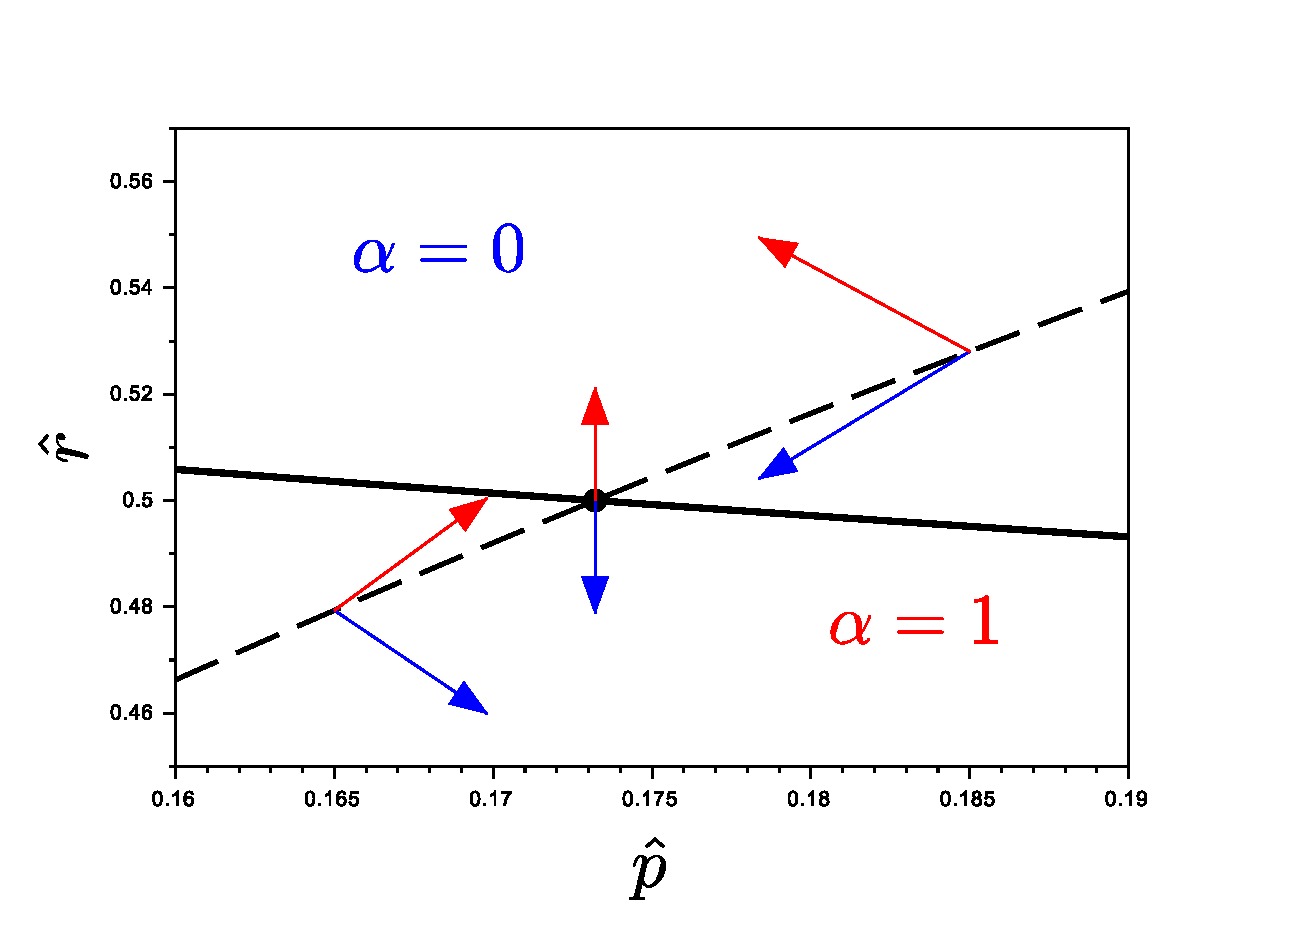
\includegraphics[width=0.8\textwidth]{Fig/Fig_sliding.eps}
\caption
{
\tr{
\textbf{Local stability of the on-off strategy.}
The on-off strategy sets $\alpha$ to a value of 0 (1) when $\hat{r} > g(\hat{p})$ ($\hat{r} < g(\hat{p})$).
The solid, black curve is the $\hat{p}$-nullcline.
The dashed, black curve is the curve $\hat{r}=g(\hat{p})$.
The arrows represent the vector fields for $\alpha=0$ (in blue) and $\alpha=1$ (in red).
The intersection of the $\hat{p}$-nullcline and the curve $\hat{r}=g(\hat{p})$ corresponds to a unique non-trivial stable steady state, which is equal to $(\hat{p}_{opt}^*, \hat{r}_{opt}^*)$ by Eq.~\ref{eq:supp_adim_h}.
}
}
\label{fig:sliding}
\end{figure}

}

\bibliographystyle{plos2015}
\bibliography{references}

\end{document}